% !TEX encoding = UTF-8
% !TEX TS-program = pdflatex
% !TEX root = ../tesi.tex
% !TEX spellcheck = it-IT

%**************************************************************
%\chapter{Analisi dei requisiti}
%\label{cap:analisi-requisiti}
%**************************************************************
%
%\intro{Breve introduzione al capitolo}\\
%
%\section{Casi d'uso}
%
%Per lo studio dei casi di utilizzo del prodotto sono stati creati dei diagrammi.
%I diagrammi dei casi d'uso (in inglese \emph{Use Case Diagram}) sono diagrammi di tipo uml dedicati alla descrizione delle funzioni o servizi offerti da un sistema, così come sono percepiti e utilizzati dagli attori che interagiscono col sistema stesso.
%Essendo il progetto finalizzato alla creazione di un tool per l'automazione di un processo, le interazioni da parte dell'utilizzatore devono essere ovviamente ridotte allo stretto necessario. Per questo motivo i diagrammi d'uso risultano semplici e in numero ridotto.
%
%\begin{figure}[!h] 
    %\centering 
    %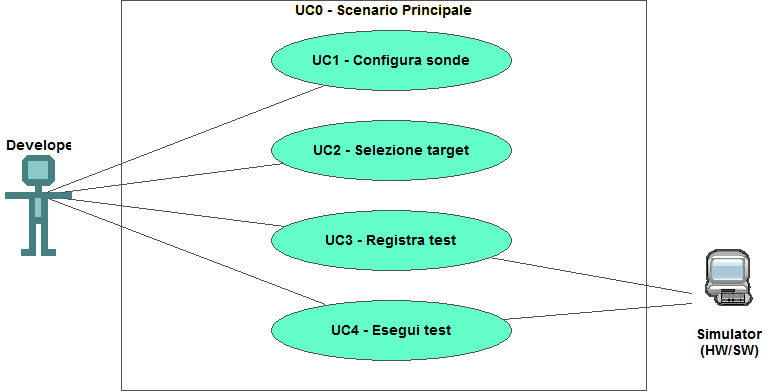
\includegraphics[width=0.9\columnwidth]{usecase/scenario-principale} 
    %\caption{Use Case - UC0: Scenario principale}
%\end{figure}
%
%\begin{usecase}{0}{Scenario principale}
%\usecaseactors{Sviluppatore applicativi}
%\usecasepre{Lo sviluppatore è entrato nel plug-in di simulazione all'interno dell'IDE}
%\usecasedesc{La finestra di simulazione mette a disposizione i comandi per configurare, registrare o eseguire un test}
%\usecasepost{Il sistema è pronto per permettere una nuova interazione}
%\label{uc:scenario-principale}
%\end{usecase}
%
%\section{Tracciamento dei requisiti}
%
%Da un'attenta analisi dei requisiti e degli use case effettuata sul progetto è stata stilata la tabella che traccia i requisiti in rapporto agli use case.\\
%Sono stati individuati diversi tipi di requisiti e si è quindi fatto utilizzo di un codice identificativo per distinguerli.\\
%Il codice dei requisiti è così strutturato R(F/Q/V)(N/D/O) dove:
%\begin{enumerate}
	%\item[R =] requisito
    %\item[F =] funzionale
    %\item[Q =] qualitativo
    %\item[V =] di vincolo
    %\item[N =] obbligatorio (necessario)
    %\item[D =] desiderabile
    %\item[Z =] opzionale
%\end{enumerate}
%Nelle tabelle \ref{tab:requisiti-funzionali}, \ref{tab:requisiti-qualitativi} e \ref{tab:requisiti-vincolo} sono riassunti i requisiti e il loro tracciamento con gli use case delineati in fase di analisi.
%
%\newpage
%
%\begin{table}%
%\caption{Tabella del tracciamento dei requisti funzionali}
%\label{tab:requisiti-funzionali}
%\begin{tabularx}{\textwidth}{lXl}
%\hline\hline
%\textbf{Requisito} & \textbf{Descrizione} & \textbf{Use Case}\\
%\hline
%RFN-1     & L'interfaccia permette di configurare il tipo di sonde del test & UC1 \\
%\hline
%\end{tabularx}
%\end{table}%
%
%\begin{table}%
%\caption{Tabella del tracciamento dei requisiti qualitativi}
%\label{tab:requisiti-qualitativi}
%\begin{tabularx}{\textwidth}{lXl}
%\hline\hline
%\textbf{Requisito} & \textbf{Descrizione} & \textbf{Use Case}\\
%\hline
%RQD-1    & Le prestazioni del simulatore hardware deve garantire la giusta esecuzione dei test e non la generazione di falsi negativi & - \\
%\hline
%\end{tabularx}
%\end{table}%
%
%\begin{table}%
%\caption{Tabella del tracciamento dei requisiti di vincolo}
%\label{tab:requisiti-vincolo}
%\begin{tabularx}{\textwidth}{lXl}
%\hline\hline
%\textbf{Requisito} & \textbf{Descrizione} & \textbf{Use Case}\\
%\hline
%RVO-1    & La libreria per l'esecuzione dei test automatici deve essere riutilizzabile & - \\
%\hline
%\end{tabularx}
%\end{table}%
%**************************************************************
\chapter{Accenni al funzionamento di Alfresco}
\label{cap:architettura}
%**************************************************************

\intro{In questo capitolo viene esposto come creare un modulo e accenni all'architettura di Alfresco}\\

%**************************************************************
\section{Architettura di Alfresco}
Al cuore di Alfresco c'è un repository che fornisce uno spazio per i contenuti, e un ampio spettro di servizi che possono essere utilizzati dalle applicazioni per manipolare il suo contenuto. Il diagramma \ref{fig:architettura-generale} mostra l'idea alla base di Alfresco, che può essere considerato formato da tre principali componenti: la piattaforma (Platform), la User Interface (UI), e la componente di ricerca (Search), basata su Apache Lucene. Queste componenti sono implementate come applicazioni web separate.
\begin{figure}[!ht]
\centering
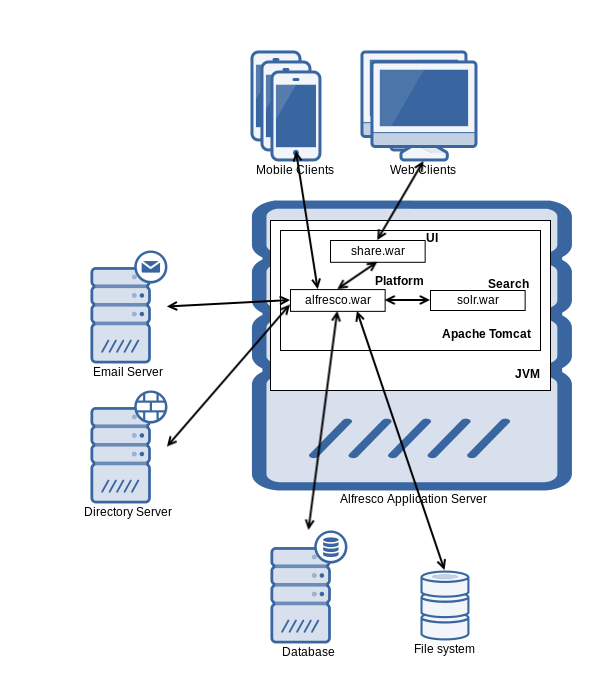
\includegraphics[width=\textwidth]{/architettura/architettura3.png}
\caption{architettura generale}
\label{fig:architettura-generale}
\end{figure}
Il principale componente è chiamato Platform ed è implementato nella web application alfresco.war. Essa fornisce il repository dove i file sono tenuti in memoria oltre a tutti i servizi di accesso e gestione collegati. Alfresco Share fornisce una interfaccia web (UI) per il repository ed è implementata nella web application share.war. Share nasce per facilitare agli utenti la gestione dei loro siti, documenti, utenti e così via.\\
La funzionalità di ricerca è implementata su Apache Solr 4 e fornisce una indicizzazione di tutti i contenuti, che rende possibile una potente funzionalità di ricerca. Oltre ai web client che accedono al repository via Share ci sono anche i dispositivi mobile che possono accedervi tramite le APIs REST fornite dalla piattaforma.

Se si approfondisce il componente Platform (contenuto nell'alfresco.war) vedremo che esso supporta i workflow nella forma dell'integrato \gls{Activiti Workflow Engine}. La piattaforma di solito, come anche nell'azienda in cui è stato svolto lo stage, viene integrata con un Directory Server (LDAP), per essere in grado di sincronizzare i gruppi e gli utenti con Alfresco Community Edition. La maggior parte delle installazioni, compresa quella di Ennova, integrano Alfresco anche con un server SMTP così il componente Platform può mandare E-mail, come ad esempio, ma non solo, inviti ai siti.

Per maggiori informazioni si rimanda alla visione della documentazione di Alfresco.

Oltre a Share vi sono anche molti altri client che possono connettersi al repository, e questi includono anche molti client compatibili con CMIS, e via il protocollo SharePoint e il client SharePoint. Esiste anche, a pagamento, la possibilità di sincronizzare i contenuti nel cloud.

Platform inoltre contiene numerose APIs, Servizi, e protocolli.

Il diagramma \ref{fig:architettura-estesa} illustra questa architettura estesa.

\begin{figure}[!ht]
\centering
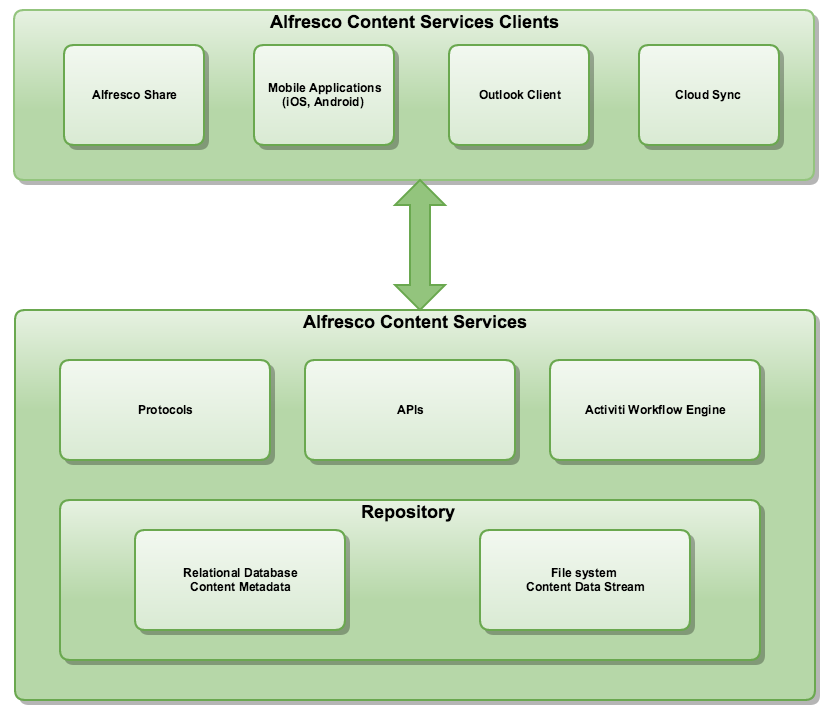
\includegraphics[width=\textwidth]{/architettura/architettura2.png}
\caption{architettura estesa\label{fig:architettura-estesa}}
\end{figure}

Si noti come i metadati del contenuto sono conservati in un database relazionale come PostgreSQL, MySQL, Oracle, e così via. Il contenuto in se è conservato nel file system (o altri sistemi di storage come Amazon S3).

Alfresco fornisce un buon numero di punti di estensione per permettere ad uno sviluppatore di customizzarlo. Questi punti hanno molte forme, tra cui:
\begin{itemize}
\item Platform extension points, illustrati nell'immagine \ref{fig:dev-platform-integration-architecture.png}
\item Share extension points, illustrati nell'immagine \ref{fig:dev-extensions-share-architecture}
\item Platform integration points, illustrati nell'immagine \ref{fig:dev-repo-extension-points.png}
\item APIs
\item Protocolli
\item Servizi
\end{itemize}
\begin{figure}[!ht]
\centering
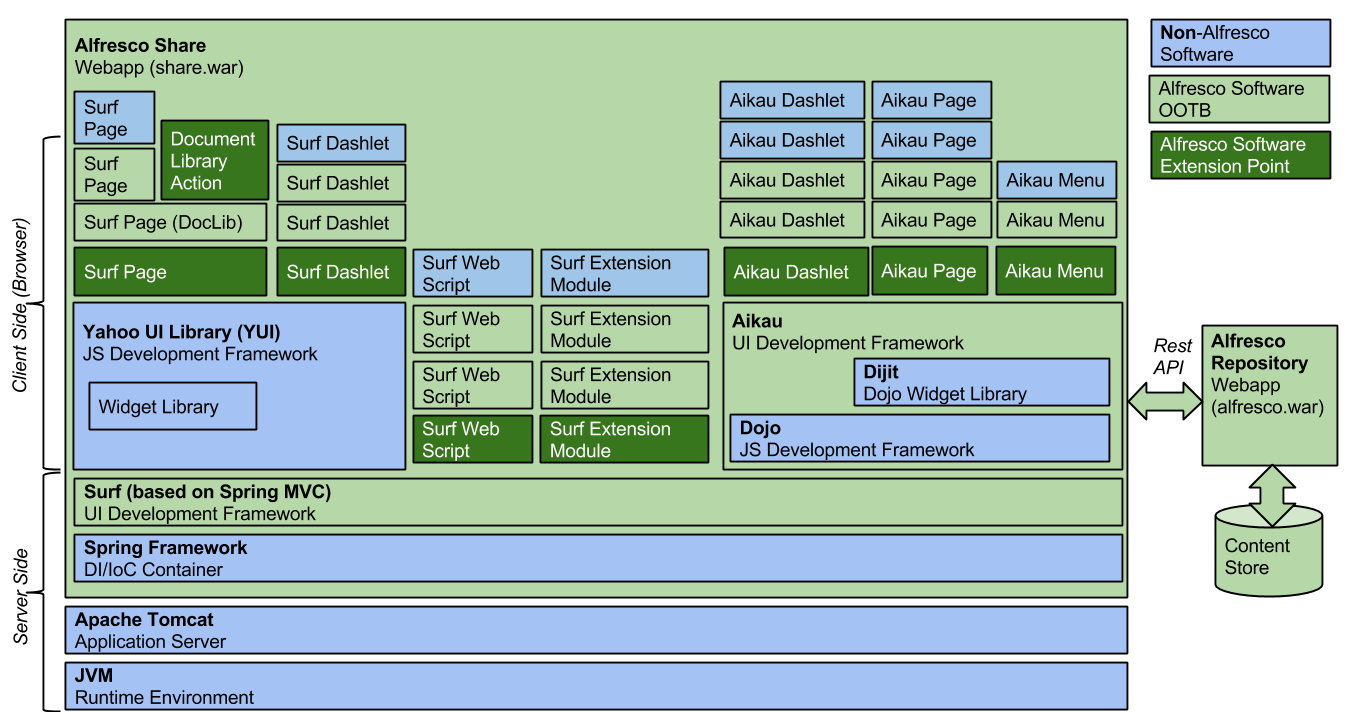
\includegraphics[width=\textwidth]{/architettura/dev-extensions-share-architecture.png}
\caption{Architettura di Share\label{fig:dev-extensions-share-architecture}}
\end{figure}
\begin{figure}[!ht]
\centering
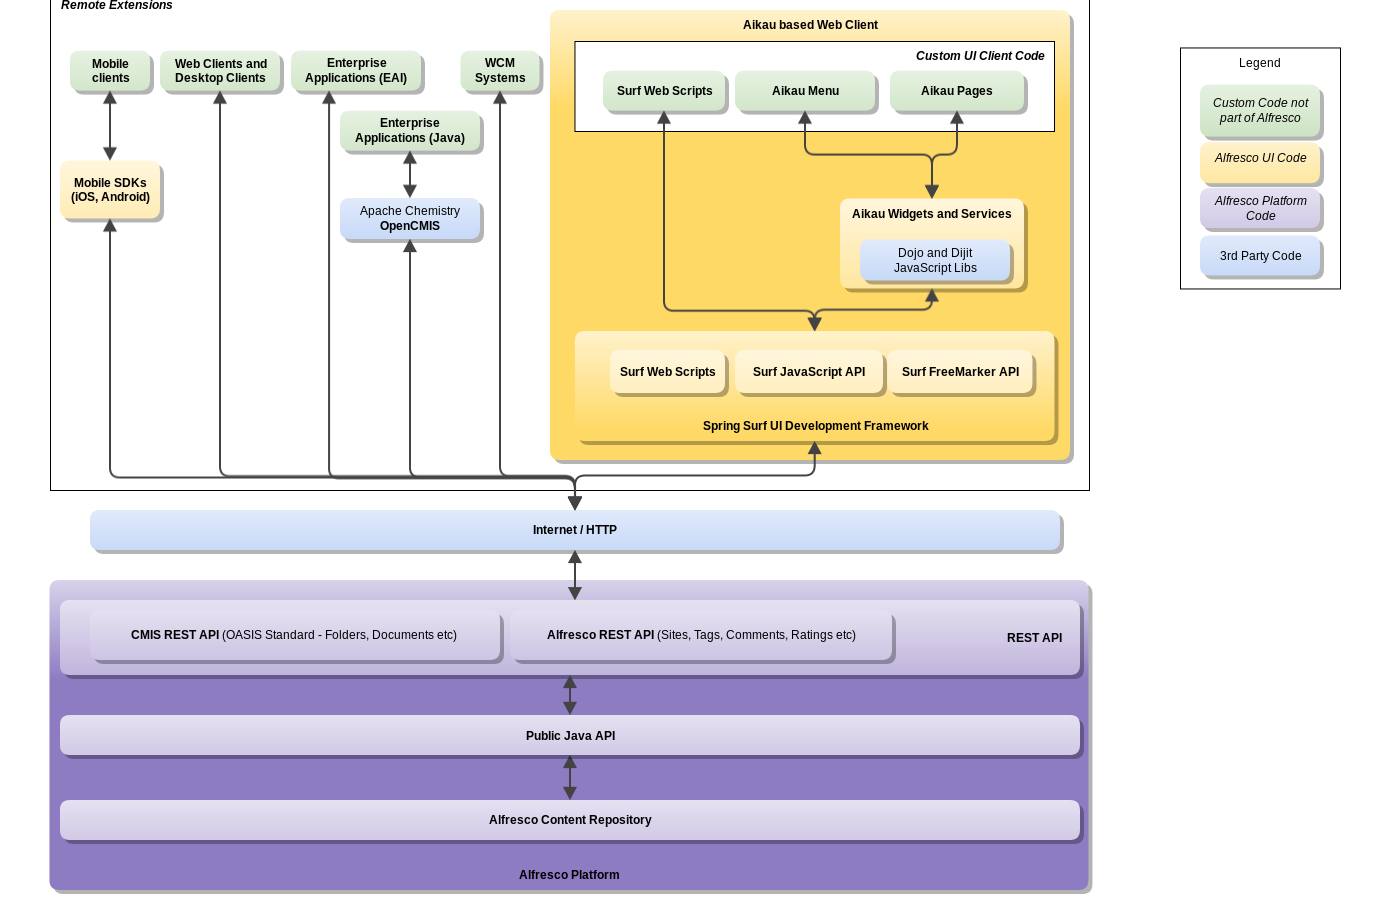
\includegraphics[width=\textwidth]{/architettura/dev-platform-integration-architecture.png}
\caption{Architettura del componente Platform\label{fig:dev-platform-integration-architecture.png}}
\end{figure}
\begin{figure}[!ht]
\centering
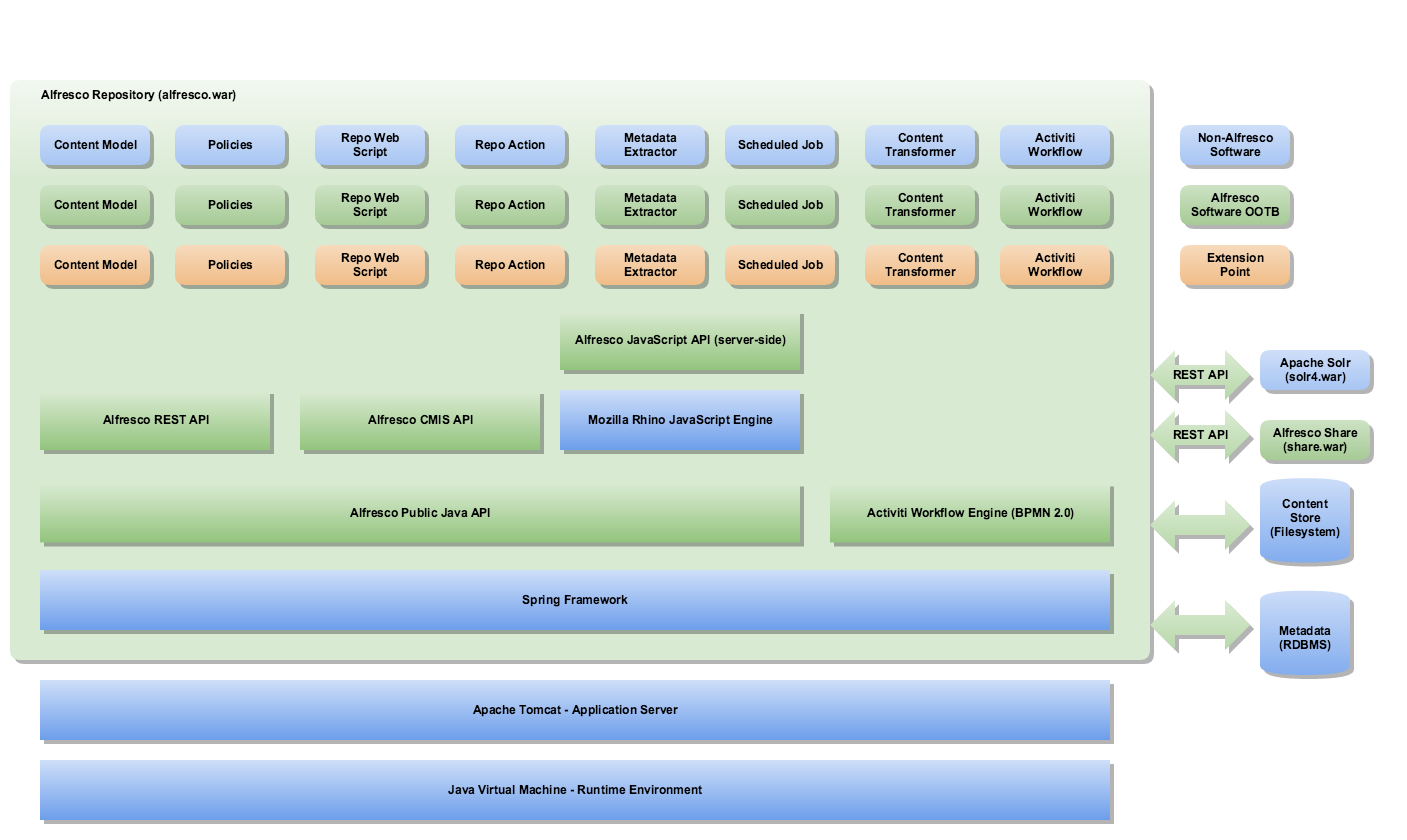
\includegraphics[width=\textwidth]{/architettura/dev-repo-extension-points.png}
\caption{Architettura del Repository\label{fig:dev-repo-extension-points.png}}
\end{figure}
\section{SDK}
L’Alfresco SDK è un kit di sviluppo basato su Maven che fornisce un approccio semplice
da utilizzare per lo sviluppo di applicazioni ed estensioni per Alfresco. Con questa SDK è
possibile sviluppare, testare, eseguire, documentare e rilasciare il proprio modulo od estensione per Alfresco. La SDK fornisce tre archetipi di Maven che possono essere
usati al fine di generare un progetto per Alfresco, e sono pensati per fornire un approccio standardizzato allo sviluppo, rilascio e distribuzione dei prodotti relativi ad Alfresco. È quindi possibile generare i
seguenti tipi di archetipi:
\begin{itemize}
\item Alfresco Repository AMP: questo archetipo si utilizza per creare moduli
per il solo Alfresco Repository Web Application;
\item Alfresco Share AMP: questo archetipo si utilizza per creare moduli per il solo
Alfresco Share Web Application;
\item Alfresco all-in-one (AIO): questo archetipo si utilizza quando vi è necessità di creare un progetto che richieda sia la componente Share che quella Repo, è la più potente e completa delle distribuzioni SDK, ma anche la più pesante.
\end{itemize}
tutti questi archetipi hanno delle caratteristiche comuni, quali:
\begin{itemize}
\item AMP packaging, cioè sono in grado di generare con la loro compilazione i file AMP, che sono i file che contengono i dati che poi verranno installati nei WAR corrispondenti.
\item La gestione delle dipendenze in Maven;
\item La generazione di uno scheletro di base sul quale poter creare il proprio progetto;
\item Il supporto ai test di unità, test che vanno inseriti in un'apposita directory.
\item Facilitazioni per l'integrazione di un progetto negli IDE, come IntelliJ IDEA e Eclipse.
\end{itemize}
\subsection{Repository AMP archetype}
L’Alfresco Repository AMP genera un scheletro di progetto per gestire le estensioni e le
personalizzazioni dell’Alfresco Repository. Questo tipo di archetipo dovrebbe essere utilizzato:
\begin{itemize}
\item  per lo sviluppo di un componente repo che non si vuole distribuire nello stesso modulo di un componente all-in-one, per facilitare il lavoro in progetti di grandi dimensioni, che così possono suddividere il progetto in componenti più piccole.
\item per poter creare un componente che sia riusabile e si possa re-includere a sua volta in componenti all-in-one.
\item per creare un modulo che vada ad interagire con la sola parte repo.
\end{itemize}
Questo archetipo presenta caratteristiche ulteriori:
\begin{itemize}
\item Ha il supporto di un database H2 per simulare il database di Alfresco.
\item supporta test di integrazione e di unità tramite Junit e RAD (rapid application development)
\end{itemize}
\subsection{Share AMP archetype}
Alfresco Share AMP Archetype genera un progetto esempio per gestire le estensioni e
le personalizzazioni di Alfresco Share. Questo tipo di archetipo dovrebbe essere utilizzato per:
\begin{itemize}
\item realizzare un modulo Share per poi includerlo all’interno di un progetto all-in-one;
\item costruire un Add-On, componente, modulo da distribuire separatamente;
\item poter spezzare il lavoro, per esempio per delegare a team diversi il lato front-end e il lato back-end;
\item creare temi e personalizzazioni che coinvolgano il solo lato UI.
\end{itemize}
Anche questo modulo presenta alcune caratteristiche particolari:
\begin{itemize}
\item sono presenti alcuni componenti di esempio per facilitare la creazione di nuove funzionalità
\item può interfacciarsi con qualsiasi componente repo di Alfresco, previa configurazione; questo permette di poter provare in sicurezza tutte le modifiche alla UI apportate direttamente in un ambiente molto vicino a quello di produzione.
\end{itemize}
\subsection{All-in-One archetype}
All-in-One archetype è un progetto multi-modulo per personalizzare ed estendere la
Share e la Repository di Alfresco.Questo tipo di archetipo dovrebbe essere utilizzato per:
\begin{itemize}
\item realizzare un progetto che permetta la personalizzazione in contemporanea e in un singolo modulo della Share e della
Repository;
\item accedere alla suite completa dei test di regressione per la Alfresco Share UI;
\item accedere ai test funzionali basati sulla libreria Alfresco Share Page Object (PO).
\end{itemize}
Le principali caratteristiche di questo archetipo sono:
\begin{itemize}
\item inclusione semplice degli AMPs extra;
\item il supporto ad estensioni Out-of-the-box come la gestione dei records, il protocollo SharePoint, la
gestione dei Media;
\item la possibilità di personalizzare i test funzionali;
\item la replicazione di un'intera distribuzione di Alfresco, che funziona autonomamente e non ha bisogno di dipendenze aggiuntive.
\end{itemize}
Ovviamente questo archetipo è il più pesante, e il suo completo deploy richiede una quantità di tempo non indifferente, per cui andrebbe usato solo se vi è reale necessità di utilizzare tutte le caratteristiche uniche che esso fornisce
\section{Gestione dei moduli}
\subsection{Creazione}
Per poter utilizzare l'SDK è necessario sottostare ai prerequisiti descritti nella pagina dei prerequisiti di installazione di Alfresco\footcite{site:alfresco-prerequisites}.
Fatto questo il progetto può essere importato in un IDE, ad esempio in Eclipse, seguendo le apposite guide nella documentazione di Alfresco\footcite{site:alfresco-rad}
Le cartelle su cui andremo a sviluppare saranno la repo-amp e la share-amp. La share-amp verrà utilizzata per sviluppare l’interfaccia grafica del modulo mentre la parte di repo-amp  per lo sviluppo del “back-end”, le altre folder create servono per replicare l’ambiente di Alfresco in fase di esecuzione del modulo, e quindi non ha senso lavorare su di esse.\\
È necessario installare il driver jdbc se si intende  lavorare nell’SDK interagendo con database terzi, e dato che non è incluso nell'SDK anche se presente nell'ambiente finale, va incluso seguendo quanto descritto nel forum di Alfresco \footcite{site:alfresco-jdbc}. 
Una volta fatto questo, bisogna aprire nell’IDE o anche a mano i vari file di Alfresco, seguendo quanto descritto nelle guide già citate, la cartella contenente la parte che verrà utilizzata per registrare la pagina in Alfresco share, nella cartella contenente le estensioni web e più nello specifico i webscript. %partendo dalla cartella di installazione (sono riportati gli indirizzi utilizzando i nomi dell’esempio sopra citato: %\texttt{/ alfresco-extension / acme-cms-poc / acme-cms-poc-share-amp / src / main / amp / config / alfresco / web-extension / site-webscripts / com / example / pages}
% (questo porta a dove è situata la pagina dimostrativa). È sufficiente fermarsi due o tre livelli sopra se l’intenzione è quella di mettere la gerarchia per una pagina custom (come fatto in questo progetto).
Una pagina fatta in alfresco share è composta da tre file, per semplicità prendiamo in considerazione la pagina di esempio già fornita:
\begin{itemize}
\item un file .xml, che descrive i dati essenziali della pagina, come quello riportato come esempio nel listato \ref{lst:codesempio}
\begin{lstlisting}[language=XML, caption=codice di una pagina di esempio, label=lst:codesempio]
<webscript>
    <shortname>Simple Page</shortname>
    <description>Simple page definition</description>
    <family>Share</family>
    <authentication>user</authentication>
    <url>/simple-page</url>
</webscript>
\end{lstlisting}
molto importanti sono il tag authentication, che specifica il livello di autenticazione necessario per accedere alla pagina, e il tag url, dal momento che definisce l’indirizzo della pagina, che sarà \texttt{<ip>:port/share/page/hdp/ws<url>} (hdp genera la pagina con header e footer, dp la pagina grezza).
\item un file .html che si comporta proprio come il body di una pagina html.
\item un file .js, che serve per applicare delle modifiche via json al model.
\end{itemize}
Quanto detto è sufficiente per creare una pagina che non necessiti di interazioni con Java.

Per quanto riguarda una pagina che invece fa uso delle api di Alfresco il procedimento è più complicato: la pagina che verrà mostrata all’utente è collocata nella cartella contenente i template per i webscripts.
La pagina generata è situata all’indirizzo \texttt{<ip>:<porta>/alfresco/service<url>}.
È inoltre necessario creare un bean che fa da collegamento tra il codice java, situato appunto in una cartella specifica che contiene le classi java, e la pagina che verrà generata. Per farlo seguire quanto descritto nelle guide per la configurazione di Alfresco \footcite{site:alfresco-bean}.

\subsection{Manutenzione}
Nel momento in cui si ha l'intenzione di modificare un modulo per evenienze riguardanti aspetti grafici o logici indiretti, si dovrà aprire il modulo con un IDE a piacere, e applicare le modifiche desiderate sui file.\\
 Il risultato delle modifiche effettuate è visionabile lanciando il comando \texttt{./run.sh} una volta posizionati all’interno della cartella del modulo su linux, \texttt{run.bat} su windows, in alternativa al comando \texttt{mvn install -Prun}  o  \texttt{mvn clean install -Prun}, se è necessario anche svuotare la cache; avviato il server basterà
aprire il browser e digitare l’url : \texttt{<ip>:8080/share/page}.
Per quanto riguarda l’importazione dei moduli nell'ambiente di Alfresco vero e proprio, si dovrà lanciare il comando \texttt{mvn clean install} all'interno sempre del folder del modulo e all’interno della cartella target delle rispettive cartelle repo-amp e share-amp si creeranno un repo-amp file e uno share-amp file. Questi dovranno essere inseriti rispettivamente nelle cartelle amps e amps\_share nell'ambiente dell'Alfresco di produzione.
Per installare il modulo  è necessario lanciare il file \texttt{alfresco-community/bin/apply\_amps.bat}, oppure lanciandolo tramite il flag \texttt{-force} se si ha già un modulo con lo stesso nome che si vuole sovrascrivere.\\
\emph{Attenzione:}L’installazione dei moduli comporta un deploy che sovrascrive il contenuto delle cartelle
\texttt{tomcat/webapps/share} e \texttt{tomcat/webapps/alfresco}. Di conseguenza nel momento in cui si è andati ad effettuare delle estensioni direttamente all’interno di queste cartelle il contenuto andrà perso. Quindi prima di effettuare questa operazione è necessario fare il backup delle cartelle indicate precedentemente.

%\emph{Per comodità d’ora in poi il nome del progetto sarà indicato come AIOProject}.